\chapter{A kódvisszafejtés lépései neurális hálók segítségével}
\label{ch:decomp}

A kódvisszafejtés neurális hálók segítségével három fő lépésben történik.
Előkészítésként az Assembly kód kinyerése történik a futtatható állományból,
például az \texttt{objdump}\cite{binutils} eszköz segítségével. Ezután az Assembly
kódot szegmentáljuk, így olyan blokkokat kapunk, amik egy sor C kódnak feleltethetőek
meg. Ezek után ezekből a blokkokból előállítjuk a megfelelő C sorokat, először csak
egy sablont, ahol a változók és számliterálok még maszkolva vannak. Végül pedig ezen
C kód és az Assembly kód segítségével előállítjuk az eredeti C kódot.

\begin{figure}[H]
	\centering
	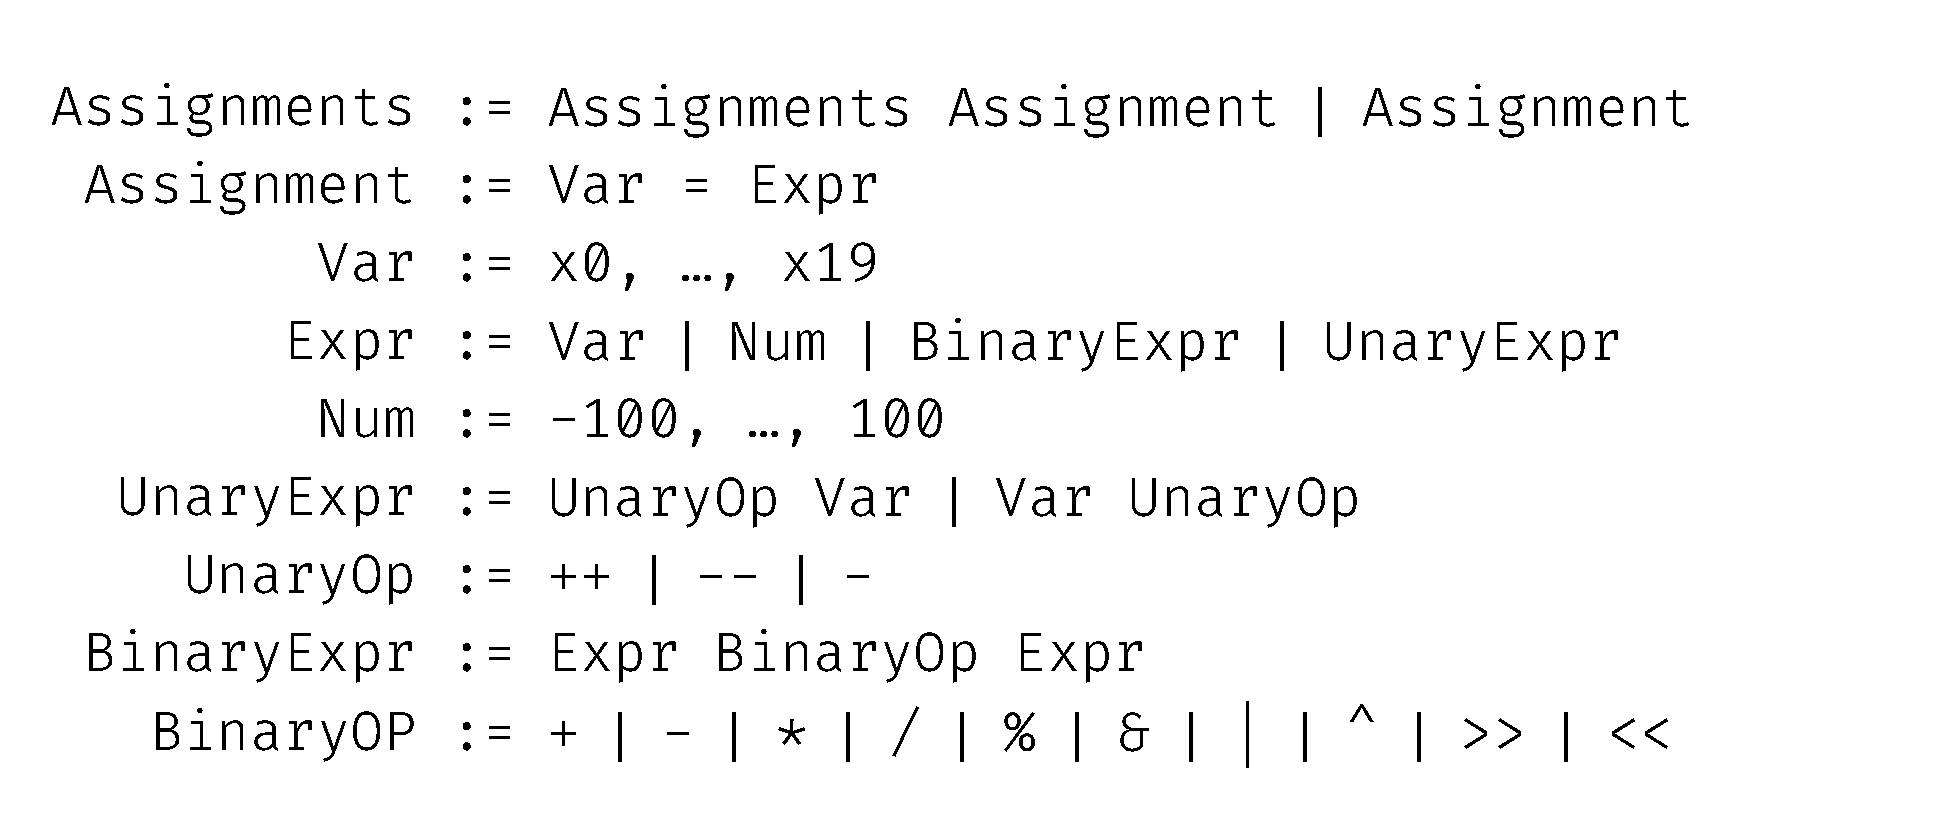
\includegraphics[width=1\textwidth,frame]{images/grammar.pdf}
	\caption{A modell tanítása során használt C kódok alapját képező nyelvtan.}
	\label{fig:grammar}
\end{figure}

\section{Assembly szegmentálás}

A visszafejtés első lépésében történik az Assembly kód szegmentálása, ahol
a cél, hogy úgy daraboljuk fel a kódot egymás utáni blokkokra, hogy egy-egy ilyen blokk egy
sor C kódnak feleljen meg. Ezt a feladatot egy \texttt{LSTM}\cite{lstm} cellákból álló
rekurrens neurális háló felhasználásával tudjuk megoldani. A modell bemenete az Assembly sorok,
a kimenete pedig minden sorra $1$, ha ott kezdődik egy blokk, $0$ egyébként. Ez
egy bináris klasszifikációs probléma, melyet a modell könnyedén megtanulhat.

\begin{figure}[H]
	\centering
	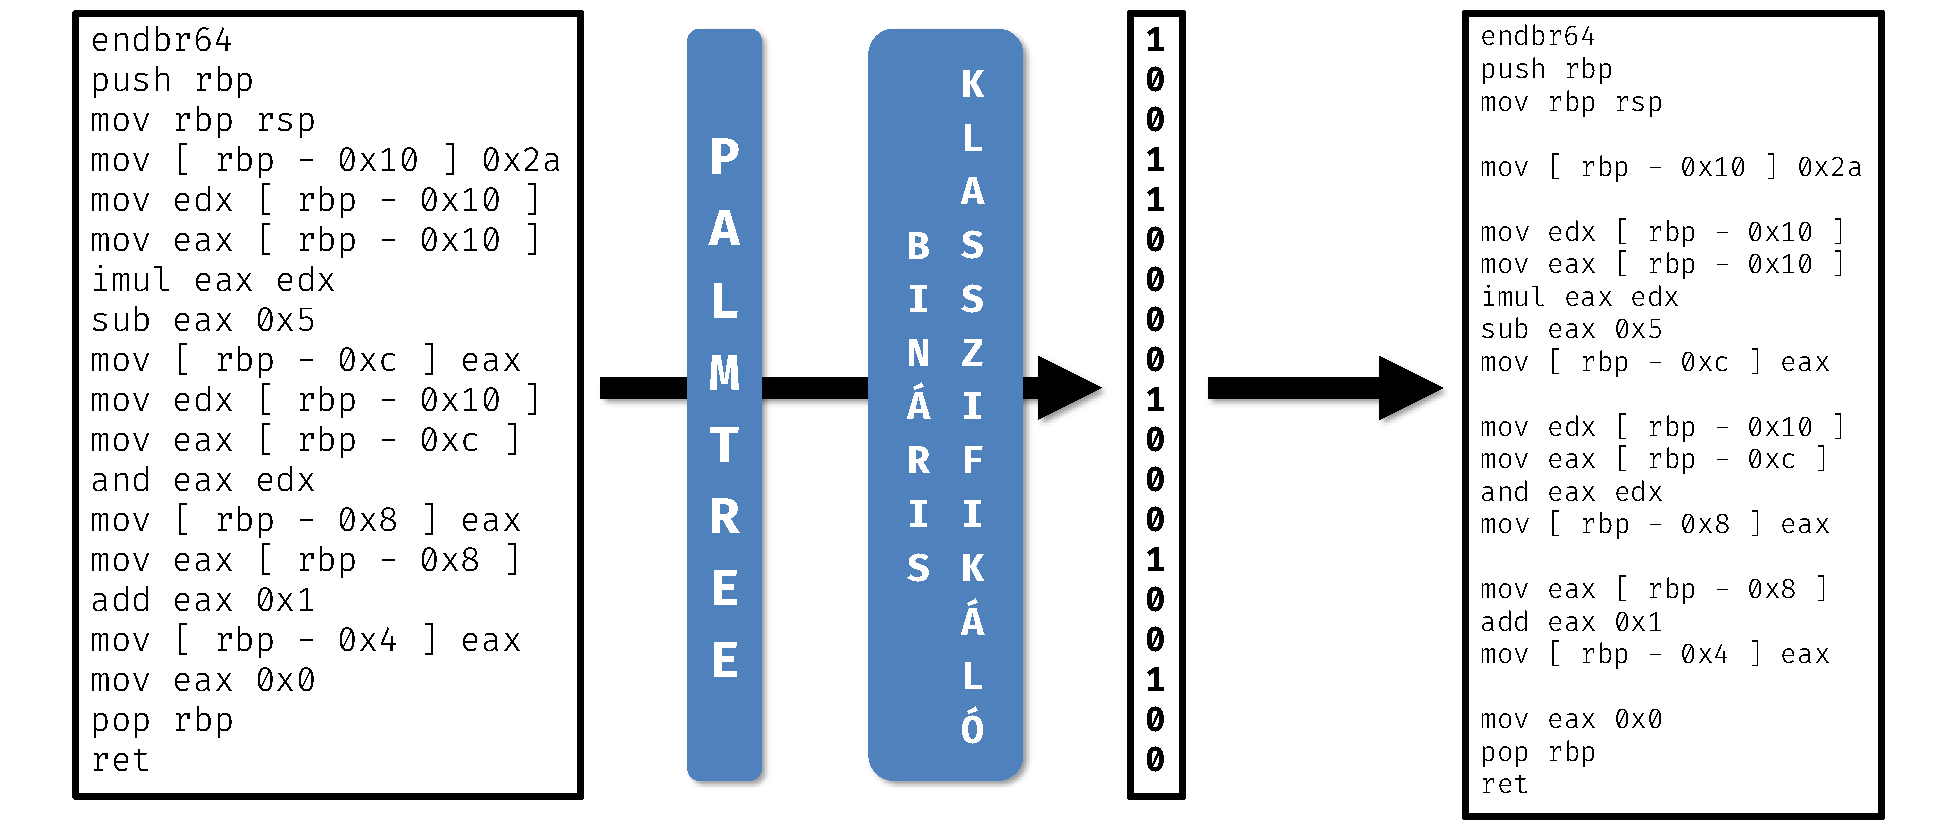
\includegraphics[width=1\textwidth]{images/segmentation_fig.pdf}
	\caption{A szegmentálás folyamata}
	\label{fig:segmentation_fig}
\end{figure}

\section{Maszkolt C kód előállítása}
A második lépésben minden Assembly blokkot egy sor C kódnak próbálunk
megfeleltetni. Fontos, hogy ebben a lépésben nem várjuk el a változók és
a számliterálok pontos visszaállítását. Ezért az eredeti C kódban minden
változó előfordulást \texttt{VAR}-ra, minden számliterál előfordulást
\texttt{NUM}-ra cserélünk. A konkrét értékek visszahelyettesítése majd
a harmadik lépésben fog megtörténni.

Ezt a problémát egy enkóder-dekóder modell segítségével oldhatjuk meg. Az enkóder
első lépésben a bemeneti Assembly blokk sorait kódolja egy vektorba, majd
a dekóder ezen vektorból állítja elő a kimeneti tokenek listáját. A lehetséges
kimeneti tokeneket és a hozzájuk tartozó alapértelmezett indexeket az alábbi ábra
tartalmazza.

\begin{figure}[H]
	\centering
	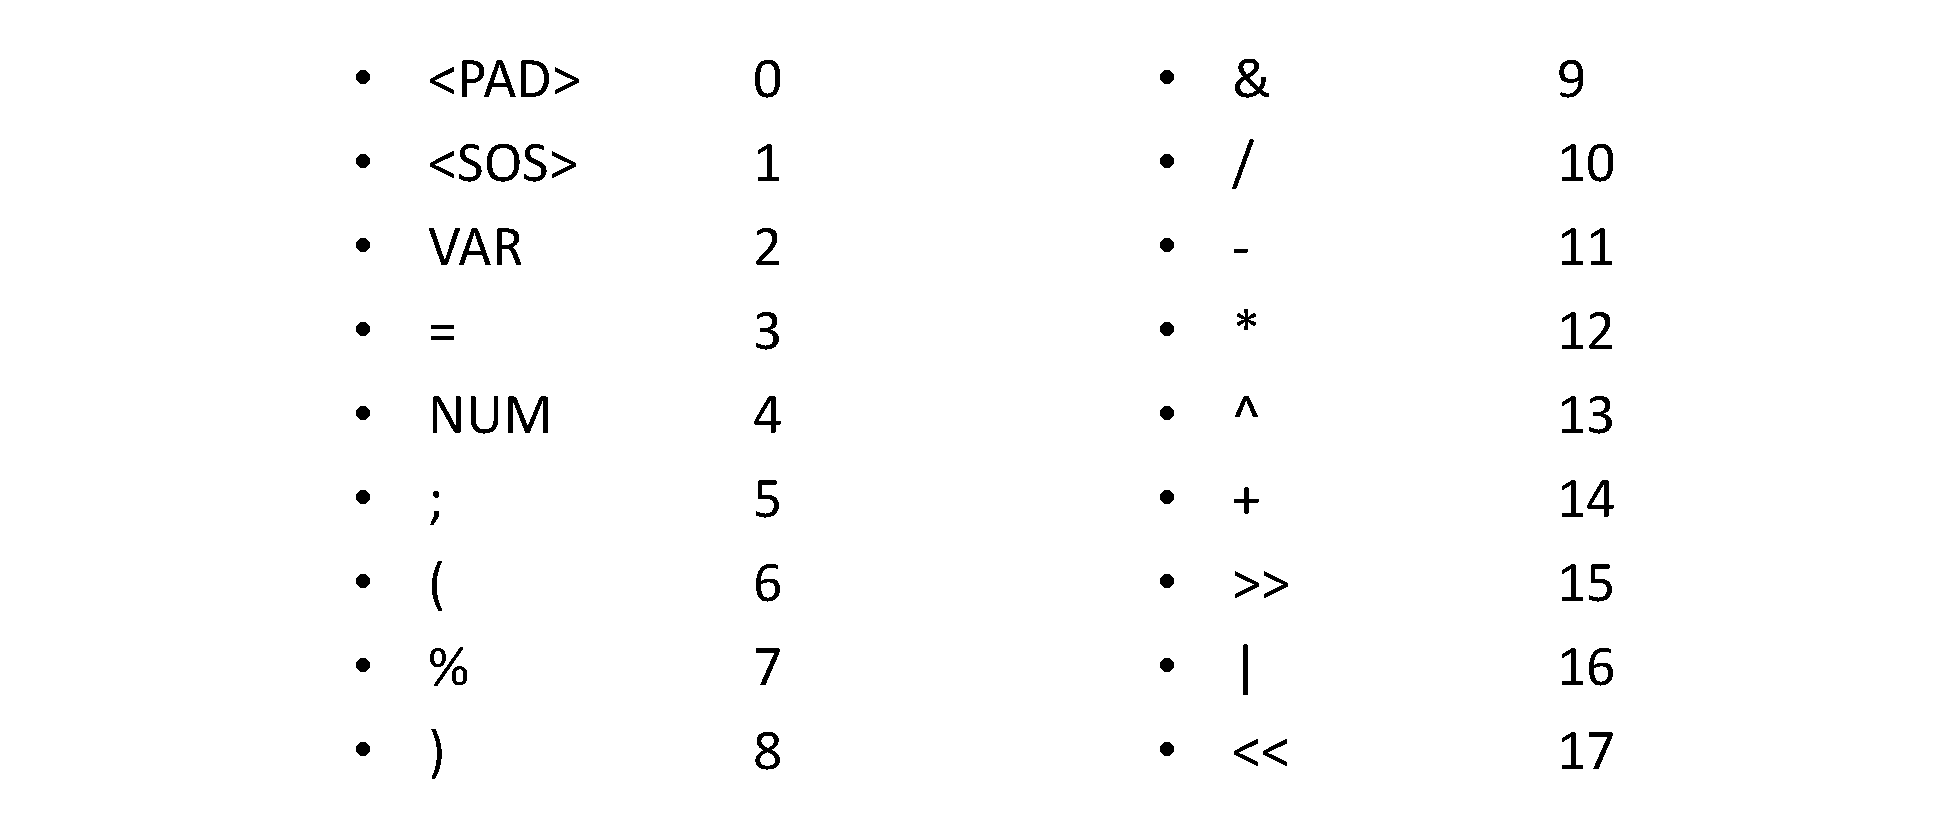
\includegraphics[width=1\textwidth,frame]{images/tokens.pdf}
	\caption{A lehetséges kimeneti tokenek és a hozzájuk tartozó alapértelmezett indexek.}
	\label{fig:tokens}
\end{figure}

\begin{figure}[H]
	\centering
	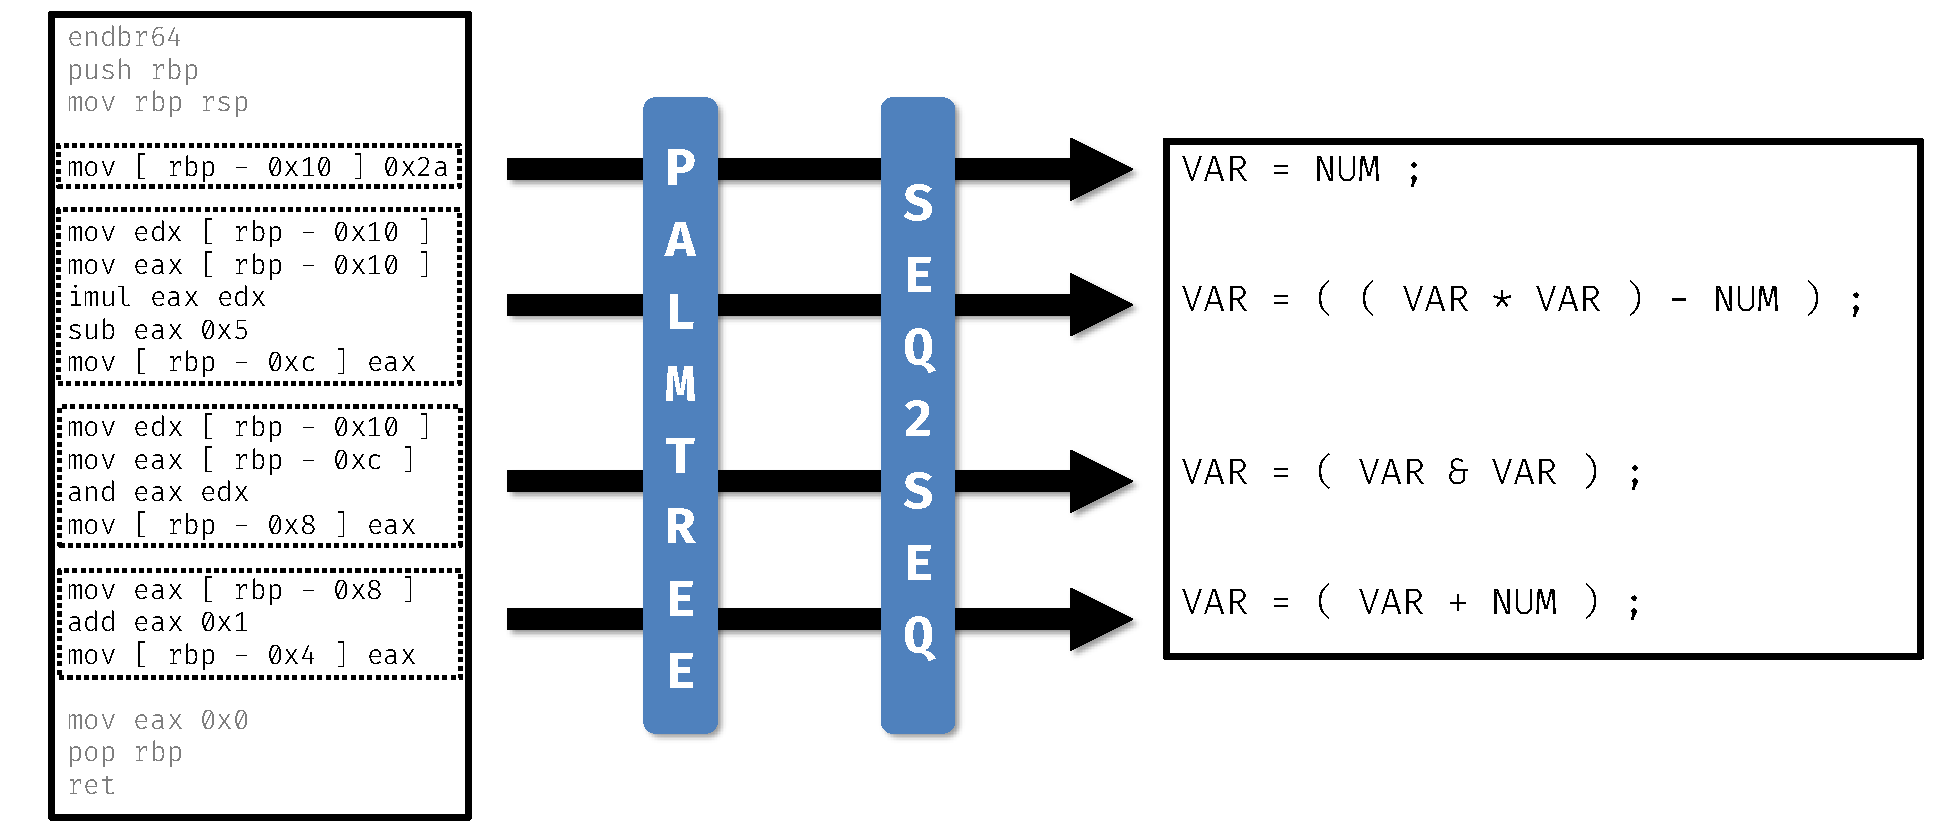
\includegraphics[width=1\textwidth]{images/translation_fig.pdf}
	\caption{A maszkolt C kód előállításának folyamata}
	\label{fig:translation_fig}
\end{figure}

\section{Változók és számliterálok rekonstruálása}
A harmadik lépésben minden előállított maszkolt C sorra megpróbáljuk
visszaállítani, hogy konkrétan milyen változók\footnote{A konkrét változónevek
elvesznek a fordítás során, így ezeket nem lehet visszafejteni, ezért itt
annyit követelünk meg, hogy két változó ugyanaz-e vagy sem.} és milyen
számliterálok szerepeltek ott. Ezeket soronként, a hozzá tartozó Assembly blokk
segítségével próbáljuk rekonstruálni, az alábbi lépésekben:
\begin{enumerate}
    \item Változók és számliterálok kinyerése a megfelelő Assembly blokkból.
    \item Ezek permutálása és behelyettesítése a \texttt{VAR} és \texttt{NUM}
    tokenek helyére.
    \item Az eddig rekonstruált és a mostani behelyettesítésből kapott kódrészlet lefordítása.
    \item Ha a lefordított Assembly megegyezik\footnote{Teljes egyezést nem
    várhatunk el, hiszen lehet, hogy pl. más regiszterekre hivatkozunk, ezért
    csak "szerkezeti" egyezést követelünk meg.} az eredeti Assembly-vel, akkor
    lépünk a következő blokkra, különben visszalépünk a $2.$ pontra.
\end{enumerate}
Így sorról sorra behelyettesítjük a változókat és számliterálokat, míg végül
visszanyerjük az eredeti\footnote{A változónevek $x0,x1,\dots$ lesznek}
C kódot.
\subsection{Probléma a szorzással, osztással és modulozással}
Az \texttt{x0 = x1 + 5 ;} kifejezésnek megfelelő Assembly blokkban 
megjelenik az $5$-ös számliterál, ugyanakkor ez nem minden műveletnél van így.
Hatékonysági okokból a számmal való osztás során a fordító nem osztást fog
generálni, hanem szorzást és bitshifteléseket. Ezért például a $17$-tel való
osztás során a vonatkozó Assembly blokkban megjelenő számliterálok a $(30841, 32, 3, 31)$.
Láthatjuk, hogy $17$ ezek között nincs ott, ezért hiába próbáljuk végig
a behelyettesítéskor az összes számliterált, soha nem fogjuk a megfelelő Assembly
blokkot visszakapni.

Ezen probléma megoldására előre legenerálható, hogy egy adott számmal való
osztás során milyen "varázsszámok" jelennek meg az Assembly-ben. Ezután a fenti
algoritmus még kiegészült annyiban, hogy nem csak az Assembly-ben
megjelenő számliterálokat próbáljuk behelyettesíteni a \texttt{NUM} tokenek
helyére, hanem ha pl. a $(30841, 32, 3, 31)$ számok mind szerepelnek, akkor ehhez a listához
a $17$-et is hozzávesszük.

A szorzás és modulozás során hasonló probléma lép fel, például a $(2, 3, 6)$
számokkal való szorzás esetén egyáltalán nem jelenik meg számliterál az
Assembly-ben. Így ezeket mindig hozzá kell venni a lehetséges számliterálok
listájához, ha van a kifejezésben \texttt{*} token.

A hátránya ennek a módszernek, hogy ha egy kifejezésben több \texttt{/},
\texttt{\%} vagy \texttt{*} token van, akkor a lehetséges számliterálok száma
nagyon megnő, ezáltal a program futási ideje is sokkal nagyobb lesz, mivel
minden lehetséges behelyettesítés kipróbálása során le kell fordítani
a kapott programot.

\begin{figure}[H]
	\centering
	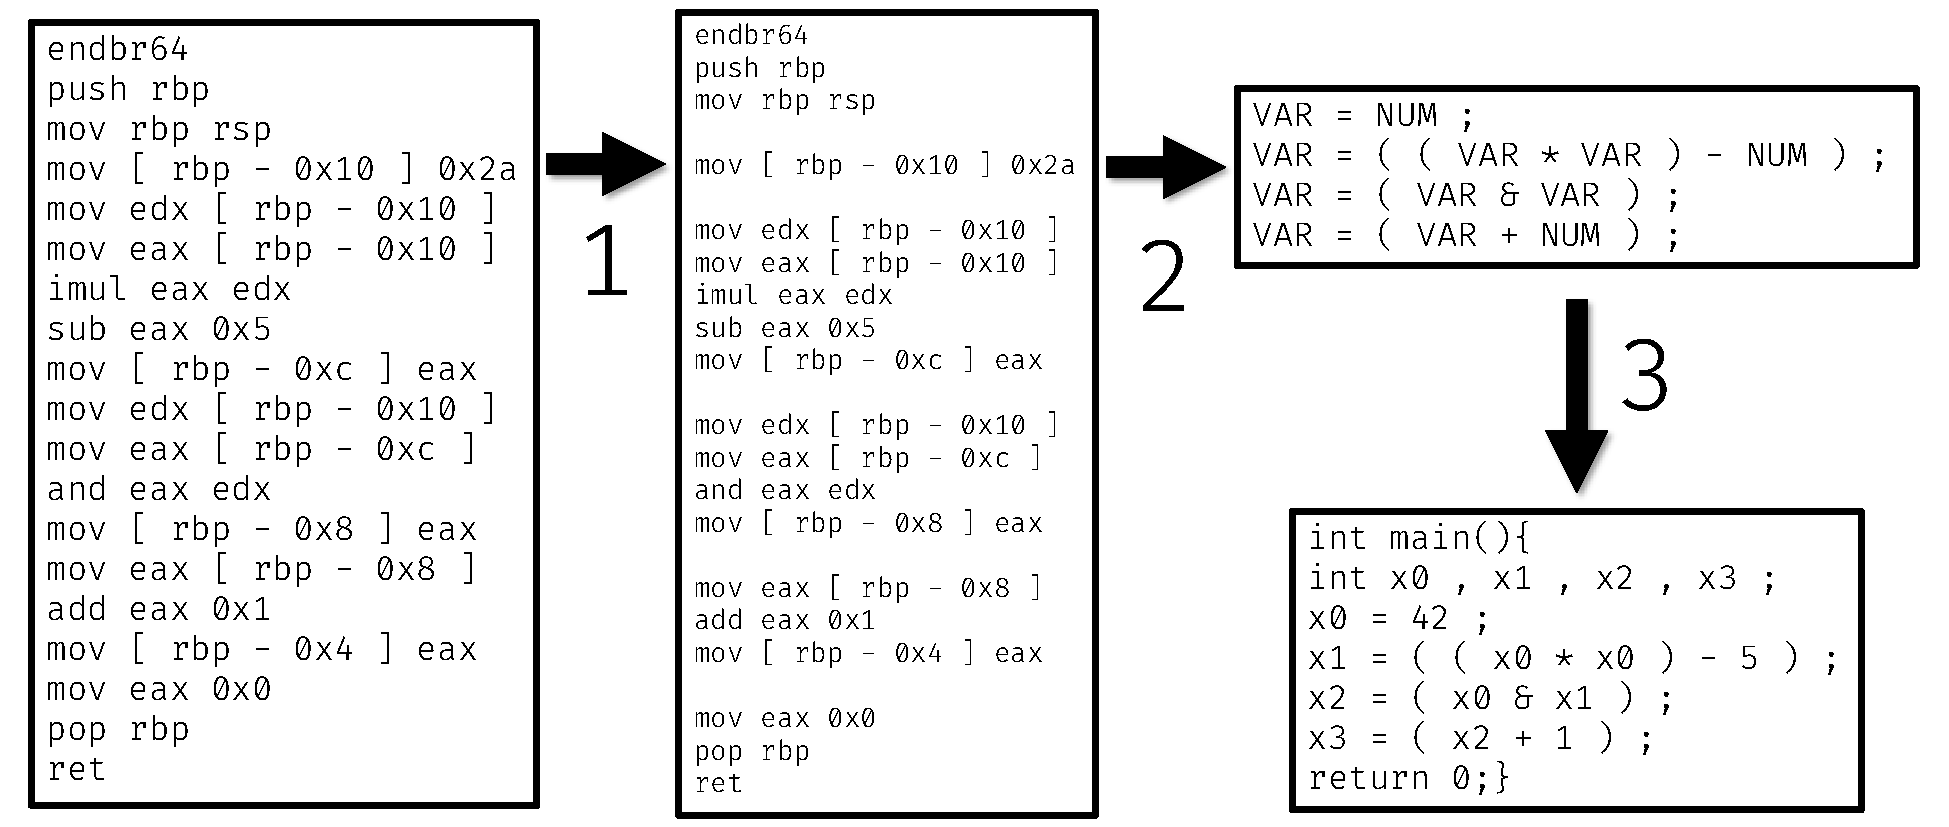
\includegraphics[width=1\textwidth]{images/steps.pdf}
	\caption{A kódvisszafejtés lépései}
	\label{fig:steps}
\end{figure}

\section{Assembly beágyazás}
Az első két lépésben használt modellek valójában nem a nyers Assembly sorokat
kapják meg bemenetként, hanem az azokból előállított kontextusvektorokat. Ez
a trükk már régóta ismert a neurális gépi fordítási problémák megoldása során,
a legismertebb ilyen megoldás a \texttt{Word2Vec}\cite{word2vec}. Ahhoz hasonlóan az
Assembly beágyazásnál is cél, hogy a hasonló soroknak közeli vektorokat
feleltessünk meg, ezzel megkönnyítve a későbbiek során a modell tanulási
folyamatát. Ezen feladat megoldására jelenleg a \texttt{Palmtree}\cite{palmtree} az egyik legjobb eszköz,
Ez minden sor Assembly-t egy \texttt{N} dimenziós vektorba képez le, működési elve
a \texttt{BERT}\cite{bert}-höz hasonló.